\chapter{Parallel computing}

\section{Introduction and basics}

If we want to improve the performance of our applications, i.e., make them run faster,
we have 3 main strategies: work harder, work smarter or get some help. The computer
engineering recipe to do so is as follows:

\begin{itemize}
    \item Use \textbf{faster hardware}: improve the operating speed of processors and other
    components. This is only constrained by the speed of light, thermodynamic laws, high
    financial costs for processor manufacture and other technical constraints.
    
    \item \textbf{Optimize algorithms} and techniques used to solve computational tasks.
    
    \item use \textbf{multiple computers/cores} to solve a particular task: connect multiple
    processors (or cores) together and coordinate their computational efforts.
\end{itemize}

The last point is the one we will focus on in this chapter. This is the core concept of
\textbf{parallel computing}.

\subsection{What is parallel computing?}

The concept of \textbf{parallelism} refers to applying \textbf{multiple processor units (PUs)}
to a single problem. To do this, we:

\begin{itemize}
    \item \textbf{Decompose} the computation into many pieces.
    \item \textbf{Assign} these pieces to different PUs.
\end{itemize}

The goal is to solve the problem faster than with a single PU. A \textbf{parallel computer}
(or system), is a computer that contains multiple PUs, such that each of them work on its 
section of the problem, and can exchange information with other PUs.

\subsection{Parallel computing vs. Serial computing}

There are two main advantages of using parallel computing over serial computing. These 
are:

\begin{itemize}
    \item \textbf{Total performance}
    \item \textbf{Total memory}
\end{itemize}

Parallel computers enable us to solve problems that benefit from (or require) a fast solution,
or that require more memory than a single computer can provide. There are examples of problems
that require both conditions to be met, such as: weather forecasting, fluid dynamic
simulations, financial simulations, etc.\\

Some specific benefits of parallel computing include:

\begin{itemize}
    \item More data points can be processed in the same amount of time: this implies
    bigger domains, bigger spatial resolution and more particles to consider.

    \item More time steps: this allows for longer runs and better temporal resolution.
    
    \item Faster execution: we can get a lower time-to-solution, and even more solutions
    in the same amount of time. This allows for larger simulations in real time.
\end{itemize}

\subsection{Examples of parallel applications}

The following is a list of some fields in which parallel computing is used:

\begin{itemize}
    \item Artificial intelligence and machine learning.
    \item Weather forecasting.
    \item Vehicle design and dynamics.
    \item Analysis of protein structures.
    \item Human genome work.
    \item Astrophysics.
    \item Earthquake wave propagation.
    \item Molecular dynamics.
    \item Climate, ocean and atmospheric modeling.
    \item Imaging and rendering.
    \item Petroleum exploration.
    \item Database query.
    \item Ozone layer monitoring.
    \item Natural language understanding.
    \item Study of chemical phenomena.
\end{itemize}

And many other scientific and industrial applications. As we can see, parallel computing
is a key technology in many fields of science and engineering.

\section{Flynn's taxonomy}

\textbf{Flynn's taxonomy} is a classification of computer architectures based on the number
of instruction streams and data streams available in the architecture. It was proposed by
Michael J. Flynn in 1966. The taxonomy is based on two concepts:

\begin{itemize}
    \item \textbf{Instruction stream}: the sequence of instructions that are executed by the
    computer.
    
    \item \textbf{Data stream}: the sequence of data that is processed by the computer.
\end{itemize}

On each type of stream, we can have one or multiple streams. This gives us four possible
combinations, which are:

\begin{itemize}
    \item \textbf{SISD}: Single Instruction, Single Data (sequential computers).
    \item \textbf{SIMD}: Single Instruction, Multiple Data.
    \item \textbf{MISD}: Multiple Instruction, Single Data (non-existent in practice).
    \item \textbf{MIMD}: Multiple Instruction, Multiple Data (most common and general parallel machine).
\end{itemize}

\begin{figure}[H]
    \centering
    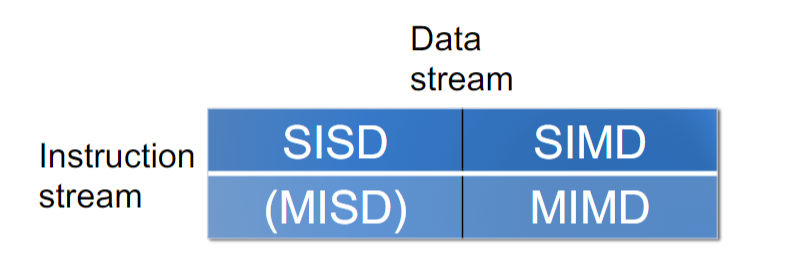
\includegraphics[width=0.7\textwidth]{figures/Flynn_tax.png}
    \caption{Flynn's taxonomy}
    \label{fig:flynn_tax}
\end{figure}

\subsection{SISD: conventional computers}

\textbf{SISD} stands for Single Instruction, Single Data. This is the most common type of
computer architecture, and it is the one we have been using so far. In this type of
architecture, a single processor executes a single instruction stream to operate on data
stored in a single memory. This is the traditional von Neumann architecture.\\

Here, the speed is limited by the rate at which the processor can execute instructions, and
transfer information internally.

\begin{figure}[H]
    \centering
    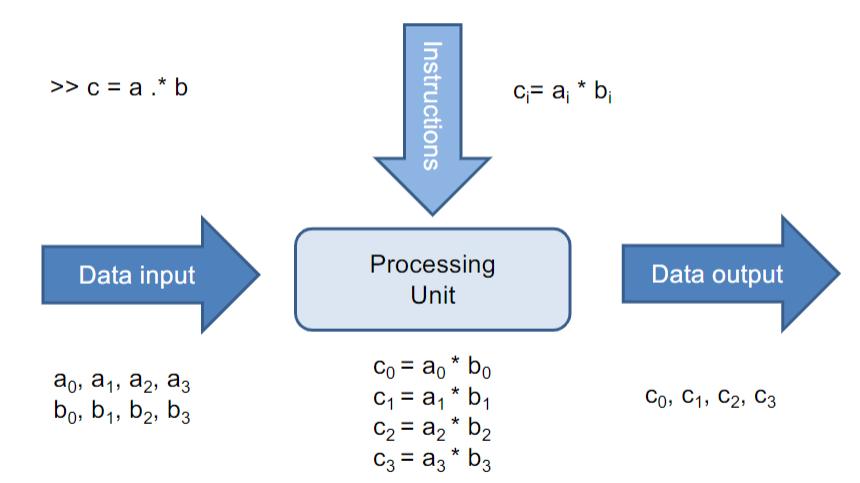
\includegraphics[width=0.7\textwidth]{figures/sisd.png}
    \caption{SISD architecture}
    \label{fig:sisd}
\end{figure}

\subsection{SIMD: vector computers}

\textbf{SIMD} stands for Single Instruction, Multiple Data. In this type of architecture,
a single instruction stream controls multiple processing elements, which operate on
multiple data streams. This is the case of vector computers.\\

In this architecture, the same operation is performed on multiple data points simultaneously.
This is useful for problems that can be parallelized, such as image processing, signal
processing, etc. SIMD relies on the regular structure of computations.

\begin{figure}[H]
    \centering
    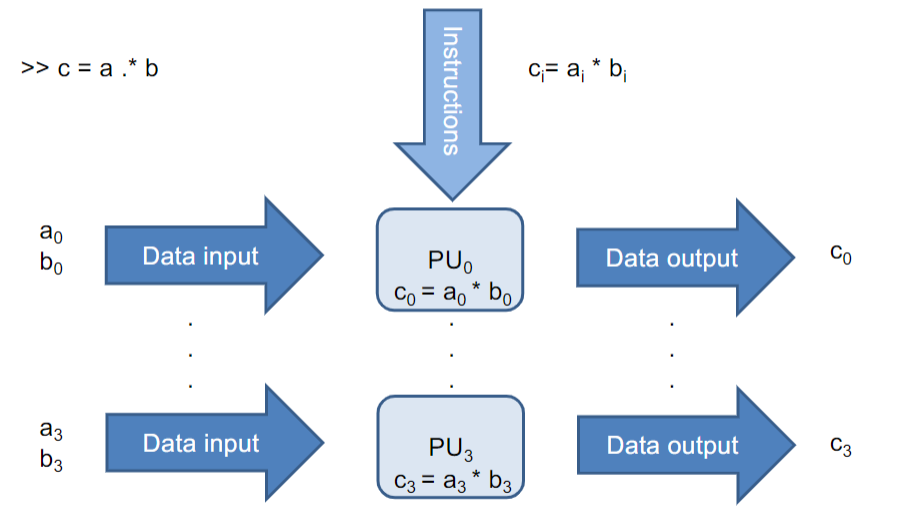
\includegraphics[width=0.7\textwidth]{figures/simd.png}
    \caption{SIMD architecture}
    \label{fig:simd}
\end{figure}

\subsection{MIMD: parallel computers}

\textbf{MIMD} stands for Multiple Instruction, Multiple Data. In this type of architecture,
multiple processors execute multiple instruction streams to operate on multiple data streams.
This is the most general type of parallel computer.\\

In this architecture, each processor can execute different instructions on different data.
This is useful for problems that are not easily parallelizable, or that require different
operations to be performed on different data points. 

\begin{figure}[H]
    \centering
    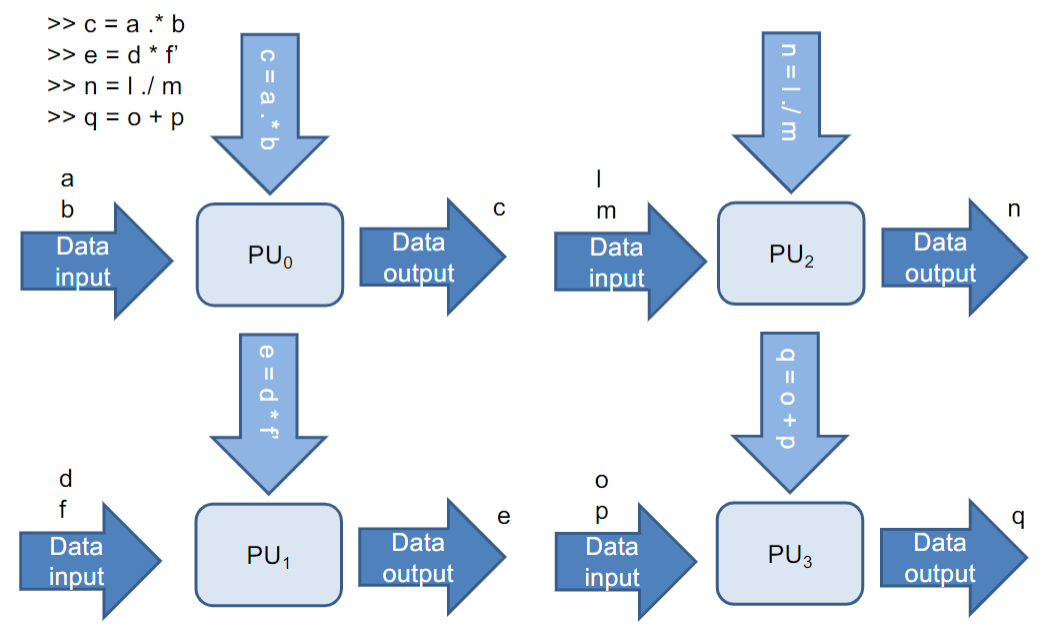
\includegraphics[width=0.7\textwidth]{figures/mimd.png}
    \caption{MIMD architecture}
    \label{fig:mimd}
\end{figure}

However, this architecture has some issues, such as:

\begin{itemize}
    \item Data distribution and dependencies.
    \item Synchonization.
    \item Communication cost.
\end{itemize}

There are two main types of MIMD architectures:

\begin{itemize}
    \item \textbf{Shared memory}: all processors share a common memory space. 
    Processor-to-processor data transfers are done using this shared memory. It has
    scalability limits. There are 2 methods for memory access: by \textbf{bus} or by
    \textbf{crossbar}.

    \begin{figure}[H]
        \centering
        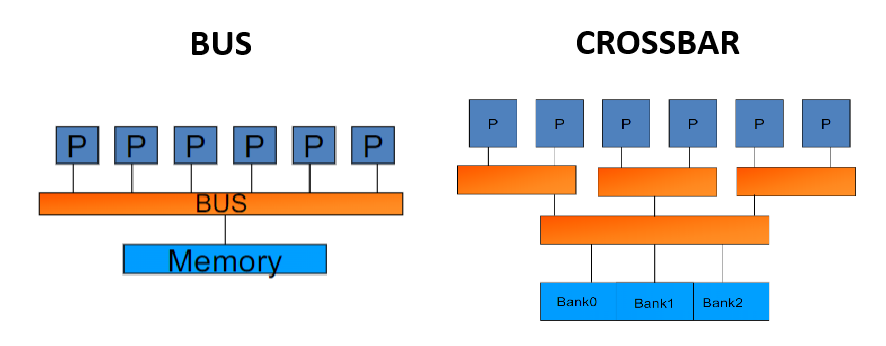
\includegraphics[width=0.9\textwidth]{figures/shared_mem.png}
        \caption{Shared memory architecture}
        \label{fig:shared_mem}
    \end{figure}

    \item \textbf{Distributed memory}: each processor has its own memory space. Processors
    must do \textbf{message passing} to exchange data between them. This architecture is more
    scalable than shared memory, but has issues like load balancing, and I/O is more
    complex.

    \begin{figure}[H]
        \centering
        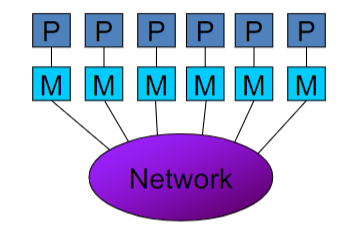
\includegraphics[width=0.5\textwidth]{figures/distrib_mem.png}
        \caption{Distributed memory architecture}
        \label{fig:dist_mem}
    \end{figure}
\end{itemize}

In this course, we will focus on \textbf{Message Passing Interface (MPI)}, that works both
on shared and distributed memory architectures.

\section{Limitations of parallel computing}

Parallel computing is not a silver bullet. There are some limitations to it, such as:

\begin{itemize}
    \item Not all problems can be parallelized: some problems are inherently sequential.
    \item There are theoretical upper limits to parallel speedup: Amdahl's law.
    \item There are also practical limits, like load balancing and non-computational
    sections (I/O, system ops, etc.).
    \item It has a different approach than sequential programming, so we need to rethink
    the algorithms and re-write the code.
\end{itemize}

\subsection{Theoretical upper limits: Amdahl's law}

We should notice that all parallel programs contain some sequential sections as well.
These sections, as well as duplicated work and no useful work done (waiting for
others), limit the parallel effectiveness:

\begin{itemize}
    \item Lots of serial computation gives bad speedup.
    \item No serial work "allows" perfect speedup.
\end{itemize}

The concept of \textbf{speedup} is defined as the ratio of the time required to run a code
on a single processor to the time required to run the same code on multiple ($N$) processors.
This is formally expressed by \textbf{Amdahl's law}:

\begin{law}[Amdahl's law]
    Let $S(N)$ be the speedup of a program running on $N$ processors. Let $f_s$ be the fraction
    of the program that is sequential, and $f_p = 1 - f_s$ be the fraction that is parallel.
    Then, the speedup is given by:

    \begin{equation}
        S(N) = \frac{1}{f_s + \frac{f_p}{N}}
    \end{equation}

    If we define $t_n$ as the time to run the program on $N$ processors, and $t_1$ as the time
    to run the program on a single processor, then the speedup can be expressed as:

    \begin{equation}
        S(N) = \frac{t_1}{t_n}
    \end{equation}

    So we get:

    \begin{equation}
        t_n = t_1 \left( f_s + \frac{f_p}{N} \right)
    \end{equation}
\end{law}

From this, we can see that it takes only a small fraction of the program to be sequential
to limit the speedup. For example, let us take a look at the following graph:

\begin{figure}[H]
    \centering
    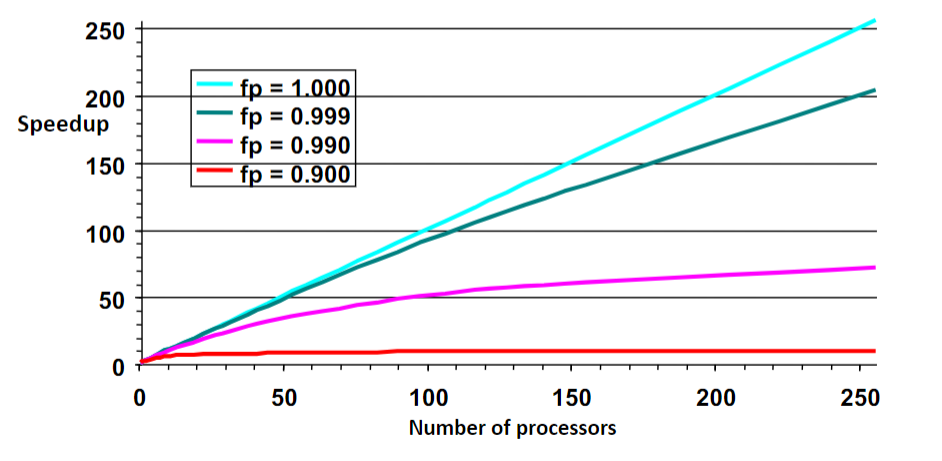
\includegraphics[width=0.7\textwidth]{figures/amdahl.png}
    \caption{Amdahl's law}
    \label{fig:amdahl}
\end{figure}

\subsubsection{Amdahl's law vs Reality}

Amdahl's law provides a theoretical upper limit to the speedup of a program, assuming 
that there is no parallelization overhead. However, in reality, overhead will result
in a further degradation of the speedup. Let us look at the following graph:

\begin{figure}[H]
    \centering
    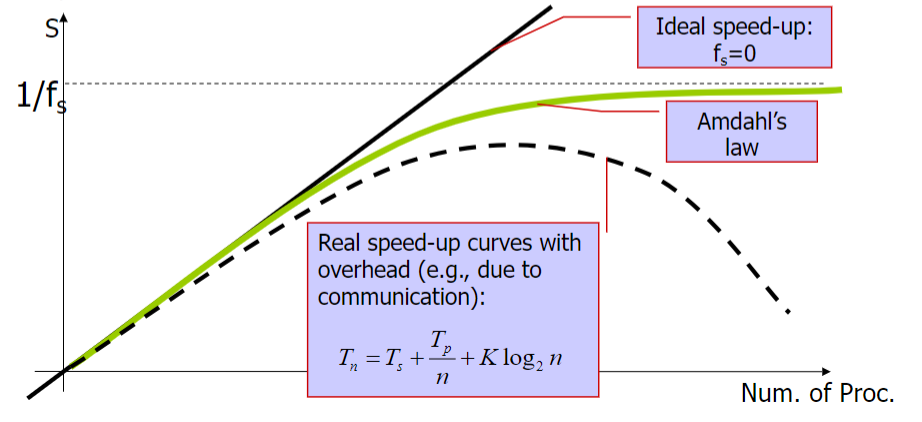
\includegraphics[width=0.95\textwidth]{figures/amdahl_reality.png}
    \caption{Amdahl's law vs Reality}
    \label{fig:amdahl_reality}
\end{figure}

\subsection{Sources of parallel overhead}

There are 3 main sources of overhead in parallel computing:

\begin{itemize}
    \item \textbf{Interprocessor communication}: time to transfer data between the processors
    is usually the most significant source of parallel processing overhead.

    \item \textbf{Load imbalance}: in some parallel applications it is impossible to 
    equally distribute the subtask workload to each processor. So, at some point, all
    but one processor might be done and waiting for the last one to complete.

    \item \textbf{Extra computation}: sometimes the best sequential algorithm is not 
    easily parallelizable and one is forced to use a parallel algorithm based on a poorer
    but easily parallelizable sequential algorithm. Sometimes, repetitive work is done
    on each of the $N$ processors, which leads to extra computation.
\end{itemize}


\subsubsection{Communication effect}

\begin{figure}[H]
    \centering
    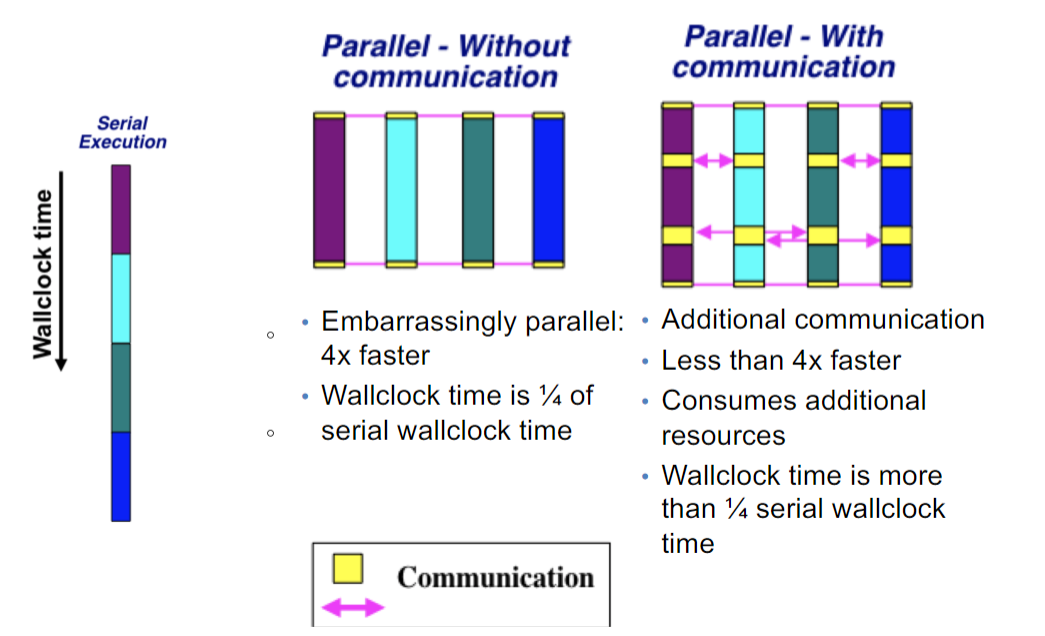
\includegraphics[width=0.5\textwidth]{figures/comm_effect.png}
    \caption{Communication effect}
    \label{fig:comm_effect}
\end{figure}

\subsubsection{Load imbalance effect}

\begin{figure}[H]
    \centering
    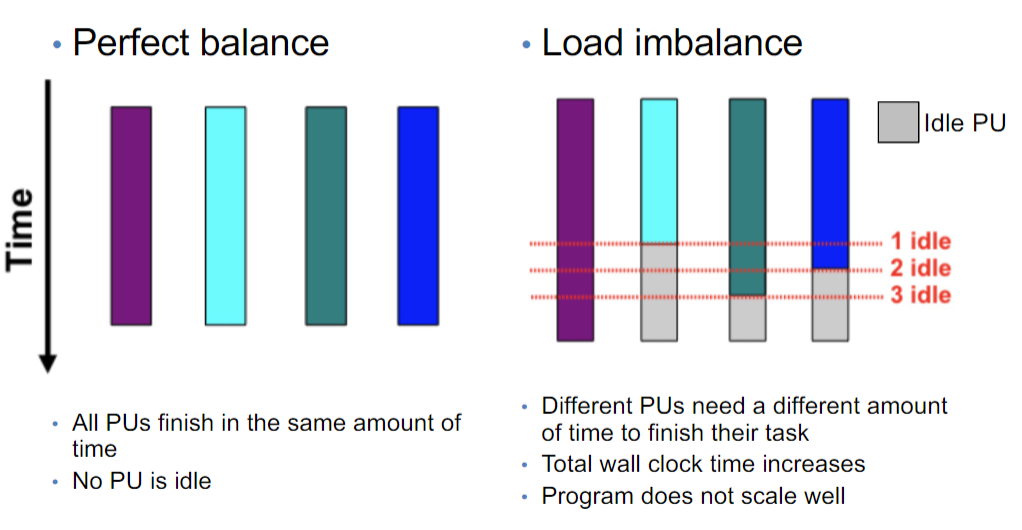
\includegraphics[width=0.5\textwidth]{figures/load_imbalance.png}
    \caption{Load imbalance effect}
    \label{fig:load_imbalance}
\end{figure}

\subsubsection{Serial performance vs parallel performance}

\begin{figure}[H]
    \centering
    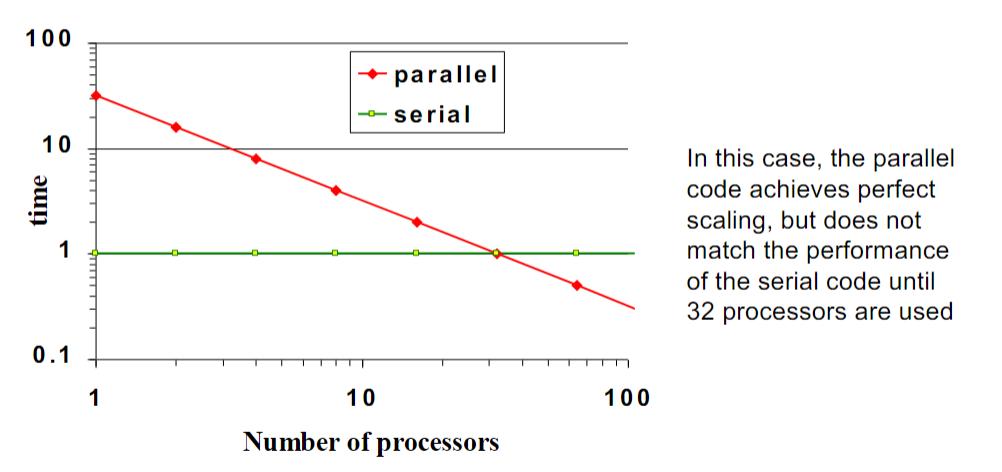
\includegraphics[width=0.5\textwidth]{figures/serial_vs_parallel.png}
    \caption{Serial performance vs parallel performance}
    \label{fig:serial_vs_parallel}
\end{figure}

\subsection{Superlinear speedup}

In some cases, we can get a superlinear speedup. This is when the speedup is greater than
the number of processors. This can happen due to:

\begin{itemize}
    \item \textbf{Caching effects}: the data fits in the cache, so the memory access is
    faster.
    
    \item \textbf{Better algorithms}: the parallel algorithm is better than the sequential
    one.
\end{itemize}

\subsection{SLOW: Starvation, Latency, Overhead, Waiting}

\textbf{SLOW} is a concept that summarizes the main issues in parallel computing:

\begin{itemize}
    \item \textbf{Starvation}: there is not enough work to do due to insufficient 
    parallelism or poor load balancing among distributed resources.
    
    \item \textbf{Latency}: waiting for access to memory or other parts of the system.
    
    \item \textbf{Overhead}: extra work that must be done to manage program concurrency
    and parallel resources, rather than the real work you want to perform. 
    
    \item \textbf{Waiting for contention}: delays due to fighting to use shared resources.
    Network bandwidth is a major constraint.
\end{itemize}

We should notice that performance enhancing comes with a price: \textbf{complexity}.
Before parallelizing a code, we should ask ourselves: is it worth our time to 
rewrite the code? Do the CPU requirements justify the parallelization? Will the code
be used enough to justify the effort?\\

In practice, writing parallel applications is hard. It requires a lot of effort, and
the results are not always as expected. We need to be careful when parallelizing
a code, and we need to be sure that the parallelization is worth the effort.\\

Sometimes, performance characteristics of applications change, and become architecture
dependent. And also, the debugging of parallel applications is harder than debugging
sequential ones.\\


\section{Examples of parallel programs}

In this section, we will see some examples of parallel programs, and how they can be
parallelized.

\subsection{Single Program, Multiple Data (SPMD)}

\textbf{SPMD} stands for Single Program, Multiple Data. This is the dominant parallel
programming model. In this model, only a single source code is written. The code can have
conditional execution based on which processor is executing the copy. All copies of 
the code are started simultaneously and communicate and synch with each other periodically.

\begin{figure}[H]
    \centering
    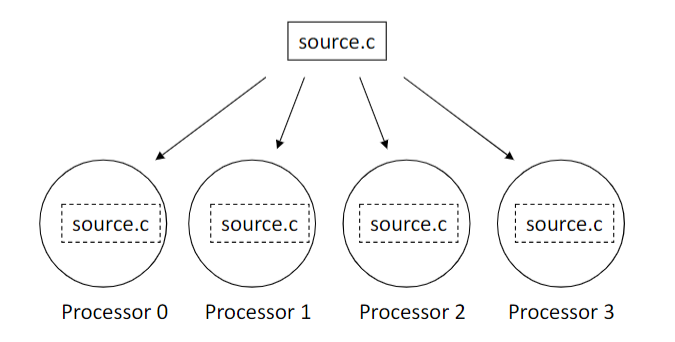
\includegraphics[width=0.7\textwidth]{figures/spmd.png}
    \caption{SPMD model}
    \label{fig:spmd}
\end{figure}

\textbf{Note:} a running program is called a \textbf{process}, and it is managed by the
operating system. 

\subsection{Basics of data parallel programming}

Let us suppose we have a simple program that runs on 2 CPUs. This program has an array
of data to be operated by both. So, to do this, the array can be split into 2 parts, and
each CPU can operate on its part. This is the basic idea of data parallel programming:

\begin{figure}[H]
    \centering
    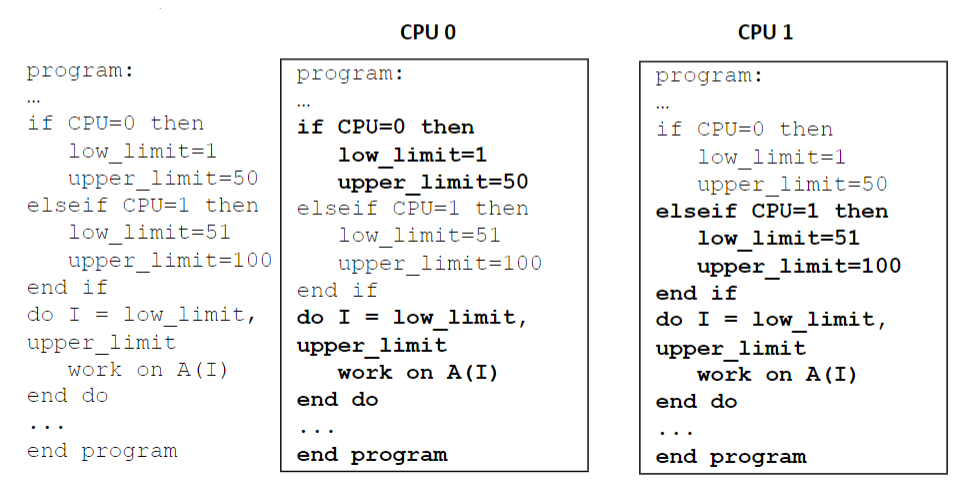
\includegraphics[width=0.7\textwidth]{figures/data_parallel.png}
    \caption{Data parallel programming}
    \label{fig:data_parallel}
\end{figure}

\subsubsection{Accessing shared variables}

If multiple processors want to write to a shared variable at the same time, there
may be conflicts. For example, let us suppose we have 2 processors that want to write
to the same variable at the same time. This can lead to the following behavior:

\begin{figure}[H]
    \centering
    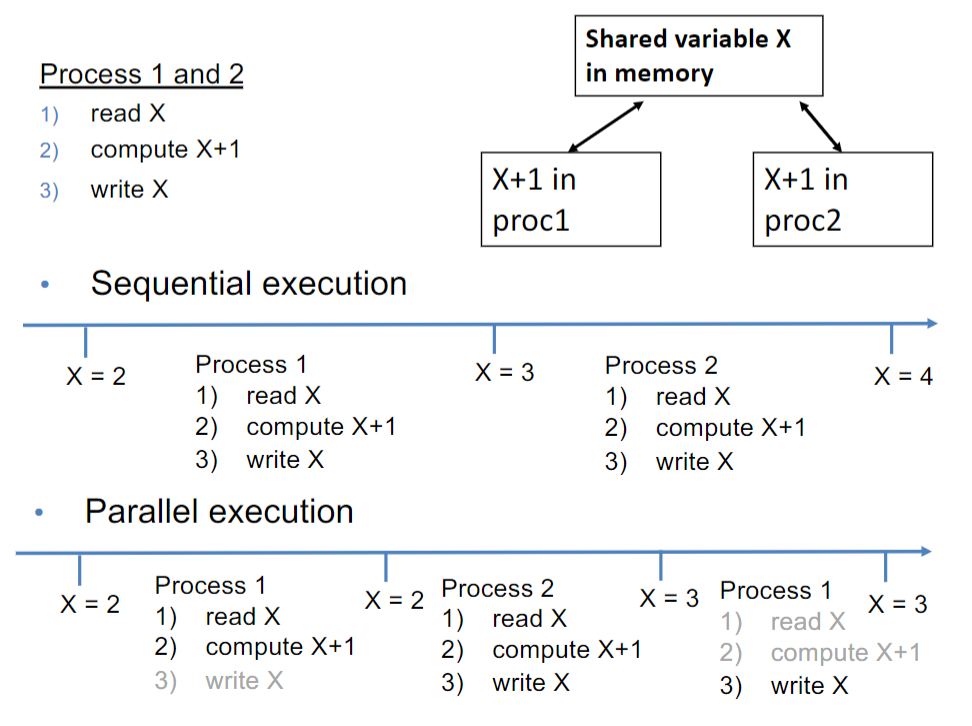
\includegraphics[width=0.7\textwidth]{figures/access_shared.png}
    \caption{Accessing shared variables}
    \label{fig:access_shared}
\end{figure}

This is known as a \textbf{race condition}. This happens when the application behavior
depends on the sequence or timing of processes which should operate properly. Critical
race conditions result un an invalid execution and bugs, as the example above.\\

To avoid this, we can use \textbf{locks}. A lock ensures mutual exclusive access to a
shared resource. When a processor wants to access the shared resource, it must first
acquire the lock. If the lock is already acquired, the processor must wait until the
lock is released. As we can see, this is another source of overhead in parallel computing.\\

\textbf{Note: beware of deadlocks!} Deadlocks occur when two or more processors are
waiting for each other to release a lock, resulting in neither of them being able to
proceed. This can be avoided by using a timeout mechanism, for example.

